\section{\label{results}Results}

\subsection{\label{fundamental_diagram} Fundamental diagram in the original model}

In Fig~\ref{fundamental_diagram_flow}, we show the fundamental diagram (density vs. flow) for different corridor widths. We can distinguish the two typical branches of the fundamental diagram. In the free flow branch ($\rho < 5$), the flow increases linearly with the density, since there are no collisions between pedestrians. In this regime, pedestrians achieve the desired velocity, leading to a flow that grows linearly with the density. That is reason why the flow takes the value of $J \sim \rho$ until $\rho=5$. This behavior applies to all the corridor width analyzed.\\

On the other hand we have the congested branch  for $\rho > 5$. Here we face two different scenarios:

\begin{itemize}
\item i) In narrow corridors (say $w < 10$) we can see that the flow reduces as the density increases. This resembles the traditional behavior of the fundamental diagram reported in the literature. 
\item ii) In wide corridors (say $w > 15$) we see that the flow increases with density. This contradicts the typical behavior of the fundamental diagram.   
\end{itemize}

Both the simulated case and the empirical results converge to a constant flow value. It is remarkable that the system does not reach a freezing state such as the one reported in Ref.\cite{kwak}. We believe that this happens because our simulated agents (as well as the empirical measurements in Ref.\cite{helbing3}) have a well defined target, the respect factor reported in Ref.\cite{parisi2} is negligible due to the circumstances and there is no reason for the individuals to stop.\\

We wonder what is the reason that determines the increase or decrease of the flow in the congested branch. Since the trajectories of pedestrians are straight (there are no crossing path that could reduce the flow), we can assert that the the friction force is the only factor in the flow reduction. The inset of the Fig.~\ref{fundamental_diagram_flow} corresponds to the empirical measures of Helbing et al. at the entrance of the Jamaraat bridge (the corridor with was $w=22$~m ) \cite{helbing3}. Notice that our simulated result corresponding to a $w=22$~m corridor, exhibit a different behavior in the congested branch. In the simulated case, the flow increases even for the greatest densities. On the contrary, the empirical measurement exhibit a flow reduction for $\rho > 5$ and it reaches a plateau for the highest density values.  \\

In order to satisfy the fundamental diagram reported in the literature, It is necessary that the flow at the maximum density ($\rho_{max} = 9$) be less than the flow at $\rho = 5$. That is:  $J(\rho = 9) < J(\rho = 5)$. From the flow definition in Eq.~\ref{ec-flow} we can derive

\begin{align*} 
v(\rho_{max}) &< \frac{5v_d}{\rho_{max}} \\
v(\rho_{max}) &< \frac{5}{9} v_d
\end{align*}

As our desired velocity is fixed $v_d = 1$~m/s, we conclude that the speed at the maximum density has to be bounded by $v(\rho_{max}) \lesssim  0.5$~m/s in order to satisfy the qualitative behavior of the fundamental diagram reported in the literature.\\

The above reasoning is consistent with the speed-density results shown in Fig.~\ref{fundamental_diagram_speed}. As a visual guide we plotted $v=0.5$~m/s with a horizontal dashed line. Pay attention to the speed values in $\rho_{max} = 9$. The values corresponding to the wider corridors ($w=15$~m and $w=22$~m) both exceed $v=0.5$~m/s. On the other hand, the values corresponding to narrower corridors fall below $v=0.5$~m/s. \\

\begin{figure}[htbp!]
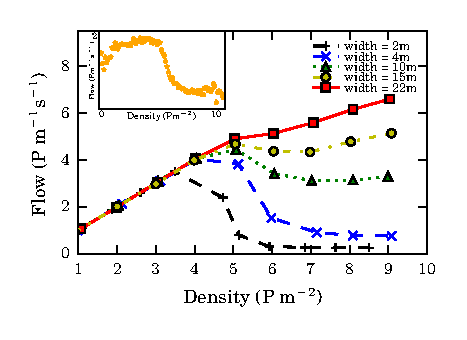
\includegraphics[width=\columnwidth]
{plots/flow-density_vd1_multiple_widths.eps}
\caption{\label{fundamental_diagram_flow} Flow as a function of the density for different widths. Initially, 
pedestrians were randomly distributed along the corridor. The measurements were taken in the middle
of the corridor once the system reached the stationary state. The length of the corridor 
was 28~m in all cases with periodic boundary conditions in the x direction.}
\end{figure}

The plots in Fig.\ref{fundamental_diagram_speed} support the fact that when the density is low enough, pedestrians manage to walk at the desired velocity ($v=1$~m/s). Only for $\rho>5$ the velocity begins the slow down proses. The inset shows the measurements at the entrance of the Jamaraat bridge. When comparing our results with the measurements of the Jamaraat bridge, it must be pointed out that the latter do not show a constant velocity for lower densities. We attribute this difference to the fact that in the real system, the pedestrian path are more complex when the density is low. Another interesting finding here is that the wider the corridor, the greater the velocity for all the density values. In Section \ref{velocity_profile} we will further discuss this topic.\\

\begin{figure}[htbp!]
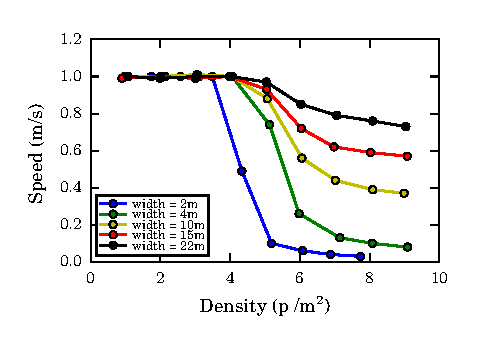
\includegraphics[width=\columnwidth]
{plots/speed-density_vd1_multiple_widths.eps}
\caption{\label{fundamental_diagram_speed} Speed as a function of the density for different widths. Initially, 
pedestrians were randomly distributed along the corridor. The measurements were taken in the middle
of the corridor once the system reached the stationary state. The length of the corridor 
was 28~m in all cases with periodic boundary conditions in the x direction.}
\end{figure}

In this subsection we have shown that the original social force model is not capable of reproducing the fundamental diagram since the flow increases even for overcrowded scenarios. 


\subsection{\label{velocity_profile} Velocity profile}

 As we mentioned in Section \ref{fundamental_diagram}, when the density is low, pedestrians achieve the desired velocity ($v=v_d=1$~m/s). Since this result is only valid for the area located in the middle of the corridor, we want to shed some light and understand what is happening in the entire corridor. In Fig.~\ref{speed-profile-w22} we show the velocity profile (velocity vs. y-location) of the pedestrians in the  corridor. We can see that low-density situations lead to a cruising velocity profile $v=v_d$. This is valid for every location in the corridor (not only the center as was previously proved). For higher densities, the velocity profile turns into a parabola-like function. This shape resembles the typical velocity profile under conditions of laminar flow in a viscous fluid, where the velocity increases toward the center of a tube. In our case, pedestrians near near the walls are the one with the lower velocity. The velocity increases when moving away from the wall until it reaches the maximum in the center of the corridor. This behavior suggests that the friction that the wall exerts on pedestrians, is playing a fundamental role in the velocity distribution. We did some simulations removing the walls and adding periodic boundary conditions in the y-coordinate. This yield to constant-cruising velocity profiles for all the densities, confirming that the walls are a necessary condition in order to produce a parabola-shaped speed profile.\\

\begin{figure}[htbp!]
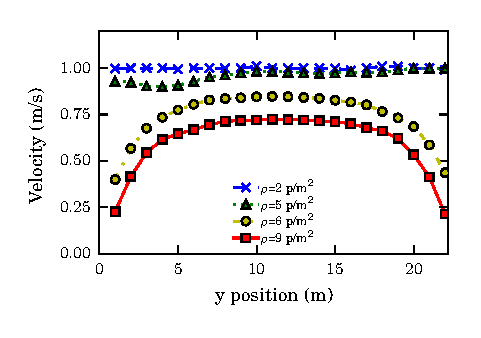
\includegraphics[width=\columnwidth]
{plots/v(y)_width22_k24.eps}
\caption{\label{speed-profile-w22} Velocity profile (velocity vs y-position) for different densities (see legend for the corresponding densities). The simulated corridor was 28~m lenght. Pedestrians walk from left to right with periodic boundary condition in the x-direction. Initially, pedestrians were randomly distributed, the corridor width was $w = 22~$m in all the cases. }
\end{figure}

In Fig.~\ref{speed-profile-multi_width} we show the velocity profile for different widths. The horizontal axis of the plot corresponds to the y-location normalized by the width of the corridor. The density chosen was $\rho = 6$ since we wanted to study a situation in which pedestrians collide with each other. Remember that when $\rho<5$, the pedestrians manage to avoid collisions. We can see the parabola shape in which the lowest velocities are in the areas near the walls. There is a clear dependence on $v_{max}$ with the corridor width. It is interesting that the wider the corridor, the higher the maximum velocity value reached.\\


\begin{figure}[htbp!]
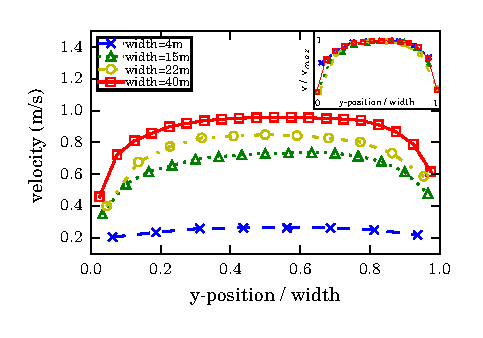
\includegraphics[width=\columnwidth]
{plots/v(y)_multi_width.eps}
\caption{\label{speed-profile-multi_width} Velocity profile (velocity vs y-position) for different corridors width (see legend for the corresponding widths). The simulated corridor was 28~m length. Pedestrians walk from left to right with periodic boundary condition in the x-direction. Initially, pedestrians were randomly distributed, the density was $\rho = 6$ in all the cases. }
\end{figure}


Fig.~\ref{speed-profile-width-normaliz} exhibits the velocity profile with the horizontal axis normalized by the corresponding corridor width (just like in Fig.~\ref{speed-profile-multi_width}). In this case, the vertical axis is normalized by the maximum velocity corresponding to each data set. Filled markers correspond density $\rho=9$, while empty markers correspond to $\rho=6$. Notice that all the data follow the same  pattern. This suggests that regardless the scale of the corridor, the velocity profile exhibits a fundamental behavior. Hence, the velocity growth rate from the wall towards the center of the corridor, is the same in spite of the size of the corridor width. 

\begin{figure}[htbp!]
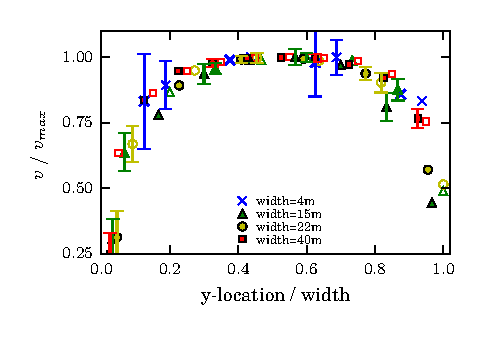
\includegraphics[width=\columnwidth]
{plots/v(y)_multi_width_normaliz.eps}
\caption{\label{speed-profile-width-normaliz} Velocity profile (velocity vs y-position) for different corridors width (see legend for the corresponding widths) and two different densities. Empty markers correspond to $\rho=6$ while filled markers correspond to  $\rho=9$. The simulated corridor was 28~m length. Pedestrians walk from left to right with periodic boundary condition in the x-direction. Initially, pedestrians were randomly distributed. The horizontal axis is normalized by the corridor width, the vertical axis is normalized by the maximum velocity attained in each case.}
\end{figure}

In this subsection we have shown that the velocity profile has a parabola shape. Pedestrians attain the maximum velocity in the middle of the corridor while the minimum is by the walls. We found out that once normalized by $v_{max}$ and the corridor width, the velocity profile yields a universal behavior (regardless the width of the corridor).\\


\subsection{Work done by friction force}

In the previous Section we have shown how the velocity takes different values along the corridor. Here we present the spacial distribution of the work done by the friction force. Only the pedestrian-pedestrian friction was calculated.\\

The work, was numerically calculated using the Trapezoidal rule on each pedestrian. The integration time step was $\Delta t = 0.05$~s. We divided the corridor into a grid with 1~m$\times$1~m cells in order to associate the work values with spacial location. In Fig.~\ref{abswg} we show three heat maps of the absolute value of the work done by the friction force. The horizontal and vertical axis represent the x location and y location of the corridor respectively. The heat map denotes higher work for red color and lower work for blue color. The walls are located at $y=0$ and $y=w$ (bottom and top of each figure). Fig.~\ref{abswg_width10} corresponds to a 10 m width corridor, Fig.~\ref{abswg_width15} corresponds to a 15 m width corridor and Fig.~\ref{abswg_width10} corresponds to a 22 m width corridor.\\

In the three figures we observe the same pattern: the regions near the walls (bottom and top) are the regions in which pedestrians suffer the higher work done by the friction. In the center of the corridor the work is reduced in all the cases. Another interesting observation is that the work seems to increase with the corridor width. This happens because in the wide corridors the relative velocity between pedestrians is greater. See Fig.~\ref{speed-profile-multi_width} and compare the slopes between the parabolas. It can be seen that the wider the corridor, the greater the slope (corresponding to locations near the wall). As it is stated in Eq.(\ref{granular}), the friction force depends on the compression and the relative velocity among pedestrians. The differences between Figs.~\ref{abswg_width10}, \ref{abswg_width15} and  \ref{abswg_width22}  are only explained by the increment of the relative velocity. The compression levels remain the same in the three cases since the compression only depends on the density (which is fix at $\rho=6$ for the three heat maps).\\

% this gives the full picture of whats going on with the velocity profile...  the interaction pedestrian-wall is friction interaction that excerts the higest friction, since the wall acts like a steady pedestrian. The pedestrian interacting with the wall fells a downward draging force.... ver explicacion vieja.. 


\begin{figure}[!htbp]
    \subfloat[]{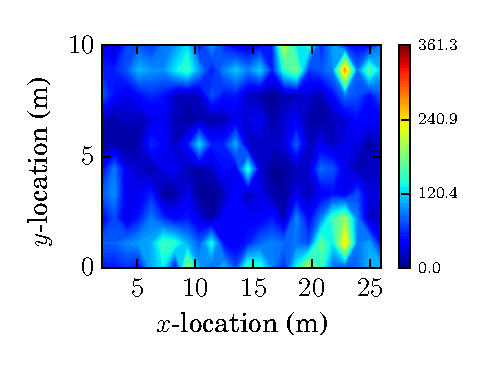
\includegraphics[width=0.47\columnwidth]{plots/abswg_width10.eps}\label{abswg_width10}}\ 
    \subfloat[]{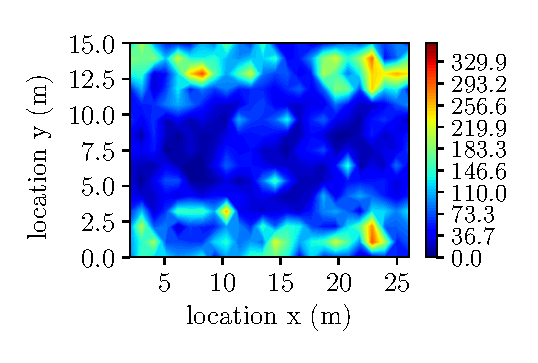
\includegraphics[width=0.47\columnwidth]{plots/abswg_width15.eps}\label{abswg_width15}}\\
    \subfloat[]{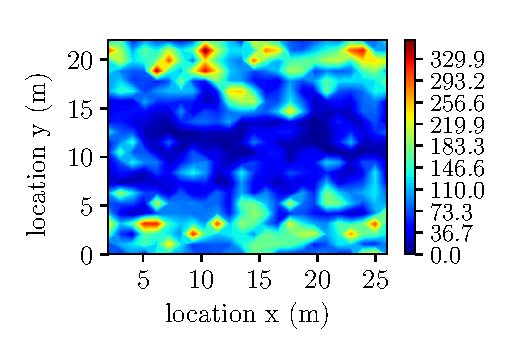
\includegraphics[width=0.47\columnwidth]{plots/abswg_width22.eps}\label{abswg_width22}}\
\caption[width=0.47\columnwidth] {Heat map for the absolute value of the work done by the friction. The axis represent the location in the corridor (x and y). The scale bar on the right is expressed in J units. The work was numerically integrated with the Trapezoidal rule with $\Delta t =0.05$~s. The pedestrians desired velocity was $v_d = 1$~m/s. The contour lines were computed on a square grid of 1~m$\times$~1m and then splined to get smooth curves.} 
 \label{abswg}
\end{figure}

In this subsection we have shown that the pedestrians in contact with the wall are the one with the higher work done by friction force. 

\subsection{Friction modification}

As already mentioned, the results shown so far indicate that friction may be the key to improving the fundamental diagram. We want to make clear that improving the fundamental diagram means obtaining the congested branch reported by different authors, in particular in the Jamaraat study of Helbing et al. where the congested branch reaches a plateau in a 22~m width corridor. The original version of the Social Force Model proposes the same friction coefficient for the pedestrian-pedestrian interaction and the pedestrian-wall interaction. The value proposed was $\kappa = 2.4\times10^{5}$. This value is widely used in many scientific papers despite it lacks a rigorous foundation. \\

We tested how the system reacts to the modification of the friction value. We define $\kappa_i$ as the friction coefficient of the pedestrian-pedestrian interaction and $\kappa_w$ as the friction coefficient of the pedestrian-wall interaction. Fig.~\ref{fgmodified-w22} shows the flow vs density for different values of $\kappa_i$ and $\kappa_w$.\\

The triangles plot in Fig.~\ref{fgmodified-w22} correspond to the increment of the wall friction in one order of magnitude (now $\kappa_w = 2.4\times10^{6}$). In this case we left the pedestrian-pedestrian friction unchanged (\textit{i.e.}, $\kappa_i = 2.4\times10^{5}$). We can see that the flow reduces a little bit, but this is not enough to produce the negative slope that characterizes the congested regime. \\

The circles correspond to a modification of the friction between pedestrians without changing the value of the wall friction. We increased the pedestrian-pedestrian friction by a factor of ten ($\kappa_i = 2.4\times10^{6}$). Here we see a significant reduction of the flow. The qualitative behavior resembles the fundamental diagram reported by Helbing et al. with a well defined congested branch for the greatest densities.\\

We also tested the case were both friction coefficients are ten times the value of the original model (now $\kappa_w = \kappa_i = 2.4\times10^{6}$). The squared symbols represent this scenario. As expected, the flow reduces significantly respect the original case (cross symbol plot). Interestingly, the reduction of the flow is more than the reduction due to the increment of $\kappa_i$ plus the reduction of the flow due to $\kappa_w$. This behavior is indicative that the superposition principle does not hold in this system because of the non-linearity of the equation of motion.   \\

This finding allows us to affirm that the friction plays a crucial role in the functional behavior of the fundamental diagram. The increment of both individual-individual friction and wall friction are determinant in order to achieve a congested branch. Other authors address the congested branch modifying different aspects of the model. Parisi et al. impose zero desired velocity once pedestrians are close enough~\cite{parisi2}, Johannson increases the relaxation time in order to slow down the net-time headway Ref.~\cite{johansson} and more recently, Kwak et al. in Ref.~\cite{kwak} induce the jamming transition by an attraction. Our results show that the empirical behavior for the fundamental diagram can be achieved by properly increasing the friction coefficients. In Appendix \ref{appendix_1} we discuss about how the modification of the relaxation time and the increment of the friction coefficient yield the same effect, since they affect the same term in the reduced-in-units equation of motion.  \\

We argue that in real scenarios, a combination of all these factors may be the cause of the marked flow reduction that portray the fundamental diagram. The pedestrians path can be very complex even if it is a simple enclosure (straight corridor) and the target is well defined (unidirectional flow). Beyond the complexities given by the internal motivations of pedestrians, we strongly suggest studying and modeling coefficients of friction between individuals and the friction with the walls. These two parameters have shown to be very important in the pedestrian dynamics and deserve a closer inspection in future research.\\

We want to emphasize that the proposals stated in Refs.~\cite{parisi2,johansson,kwak}  only apply under normal conditions. If a crowd is under high levels of anxiety (\textit{i.e.} panic), pedestrians will not keep distance with each other nor will feel the urge to see an ``attraction''. The only goal in an evacuation under panic is to leave the room. Thus, studying the friction coefficients may be a critical factor to properly reproduce the dynamics of a massive evacuation under stress.\\


\begin{figure}[htbp!]
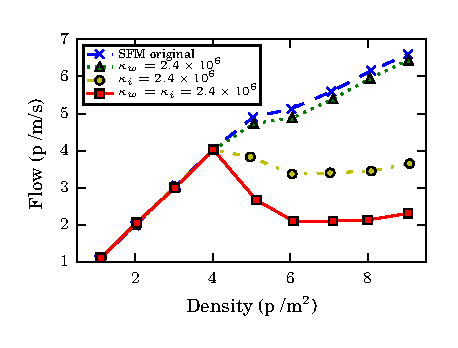
\includegraphics[width=\columnwidth]
{plots/flow-density_pasillo22m_fgmodified_multi.eps}
\caption{\label{fgmodified-w22} Fundamental diagram (flow vs density) for different friction coefficient (see legend for the corresponding values). The simulated corridor was 28~m length. Pedestrians walk from left to right with periodic boundary condition in the x-direction. Initially, pedestrians were randomly distributed. For each density, we measure the flow once the system reaches the stationary state.}
\end{figure}

In this subsection we have shown that an adequate modification of the friction coefficients yields a fundamental diagram with the qualitative behavior reported in empirical measurements (with the flow reduction for the greatest densities). We have also discussed different approaches proposed by other authors in order to attain this problem. See Appendix \ref{appendix_1} for a more detailed discussion.\\

\subsection{\label{clusters}Clusters}

Cluster formation is a very important process in pedestrian dynamics. Moreover, is the key process that explains the clogging phenomena in bottleneck evacuations. We analyzed the clustering formation according to the granular cluster definition given in~\cite{Dorso1}
In Fig.~\ref{cluster_distribution} we show the histogram of the cluster size distribution for three different densities, from top to bottom: $\rho=4.5$, $\rho=5$ and $\rho=5.5$. we have chosen these three values as lower densities yield to non-clustered arrangements and higher densities yield a unique giant cluster.     
For each density we studied two situations. The cluster size distribution for the original parameters of the Social Force Model (left hand side plots) and the cluster size distribution corresponding to the increment of the friction coefficients by a factor of ten (right hand side plots).\\

We found a couple of intriguing results. Incrementing the density produces bigger size clusters until it reaches a critical value in which the size distribution shifts to a bimodal distribution (compare \ref{size_distribution_w22_density5} with \ref{size_distribution_w22_density5_5} and \ref{size_distribution_w22_density4.5_kx10} with \ref{size_distribution_w22_density5_kx10}). Once this phenomena takes place, there are only two possibilities for the clusters: either there are many small sized clusters or there is only one giant cluster.\\

We also found that this phenomena is prompted by the friction. If the friction is higher, the transition to the bimodal distribution takes place for lower density values. See Fig.~\ref{size_distribution_w22_density5} and Fig.~\ref{size_distribution_w22_density5_kx10}. Despite the fact that both correspond to the same density,  \ref{size_distribution_w22_density5_kx10} already attained the bimodal distribution since the friction force is ten times greater than \ref{size_distribution_w22_density5}. This peculiar phenomenon occurs because when there is more friction, individuals find it more difficult to detach from each other. In the opposite case, when the friction is low, the individuals detach themselves more easily, leading to a situation where large clusters are less probable.\\

\begin{figure}[!htbp]
    \subfloat[]{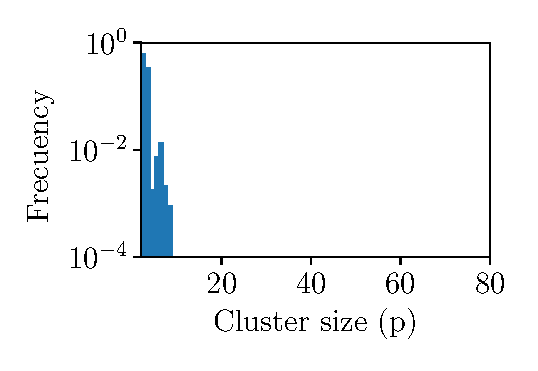
\includegraphics[width=0.47\columnwidth]{plots/size_distribution_w22_density4_5.eps}\label{size_distribution_w22_density4.5}}\ 
    \subfloat[]{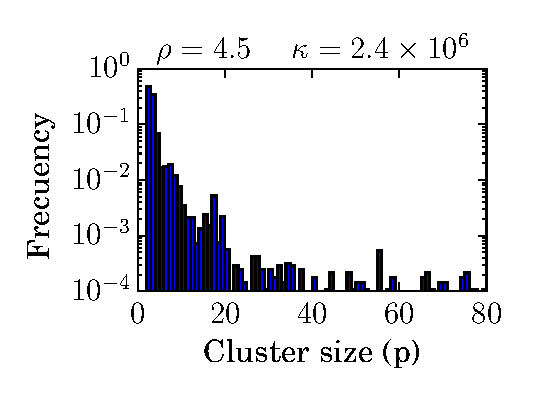
\includegraphics[width=0.47\columnwidth]{plots/size_distribution_w22_density4_5_kx10.eps}\label{size_distribution_w22_density4.5_kx10}}\\
    \subfloat[]{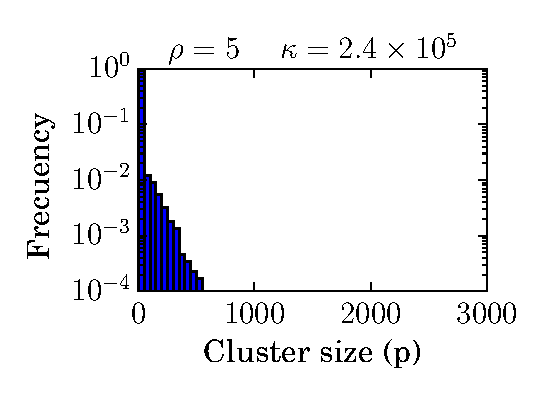
\includegraphics[width=0.47\columnwidth]{plots/size_distribution_w22_density5.eps}\label{size_distribution_w22_density5}}\
    \subfloat[]{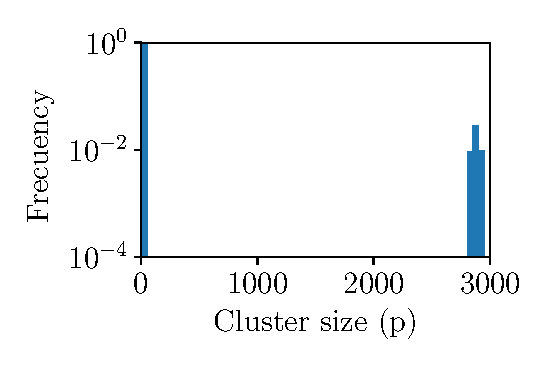
\includegraphics[width=0.47\columnwidth]{plots/size_distribution_w22_density5_kx10.eps}\label{size_distribution_w22_density5_kx10}}\\
    \subfloat[]{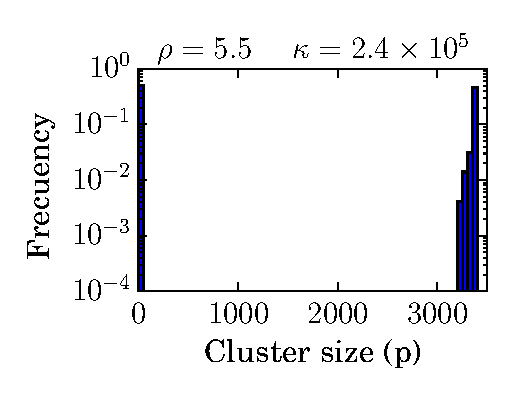
\includegraphics[width=0.47\columnwidth]{plots/size_distribution_w22_density5_5.eps}\label{size_distribution_w22_density5_5}}\
    \subfloat[]{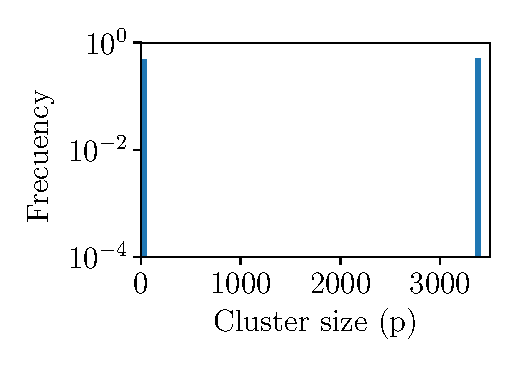
\includegraphics[width=0.47\columnwidth]{plots/size_distribution_w22_density5_5_kx10.eps}\label{size_distribution_w22_density5_5_kx10}}
\caption[width=0.47\columnwidth]{Cluster size distribution for six different scenarios. (a) SFM friction parameters and $\rho=4.5$, the bin size is 1 p (b) friction parameters increased by a factor of ten and $\rho=4.5$, the bin size is 1 p (c) SFM friction parameters and $\rho=5$, the bin size is 50 p (d) friction parameters increased by a factor of ten and $\rho=5$, the bin size is 50 p (e) SFM friction parameters and $\rho=5.5$, the bin size is 50 p (f) friction parameters increased by a factor of ten and $\rho=5.5$, the bin size is 50 p.}
\label{cluster_distribution}
\end{figure}

To understand the full picture, in Fig.~\ref{fic} we show the fraction of clustered individual as a function of the density for four different situations in which we change the friction coefficients. The fraction of clustered individuals is defined as the amount of pedestrians that belong to a cluster over the total number pedestrians in the corridor. 
We can see that there is a transition from a non-clustered crowd to a full-clustered crowd. This transition occurs for a very limited range of densities, causing the process of cluster formation to occur for $4.4<\rho<5.3$. When the friction coefficient is high, the transition takes place for lower density values. This result is consistent with the histograms shown in Fig~.\ref{cluster_distribution}, supporting the fact that friction promotes the formation of clusters. \\

As expected, the transition becomes more abrupt when both $\kappa_i$ and $\kappa_w$ are incremented (squared symbol plot). When only one of those two coefficients is incremented, the fraction of clustered individuals is greater than the original model. Notice that there is not a big difference between the modification of $\kappa_i$ and the modification of $\kappa_w$. This suggests that it does not matter if the clusterization begins to take place in the areas near the walls or in the middle of the crowd.\\


\begin{figure}[htbp!]
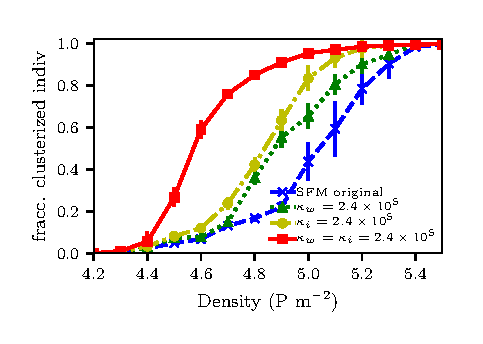
\includegraphics[width=\columnwidth]
{plots/fracc_clusteriz_vs_density.eps}
\caption{\label{fic} Fraction of clusterized individuals as a function of the density. Square symbol correspond to $\kappa_w=\kappa_i=2.4\times 10^6$, circles to $\kappa_i=2.4\times 10^6$ and $\kappa_w=2.4\times 10^5$, triangles to to $\kappa_i=2.4\times 10^5$ and $\kappa_w=2.4\times 10^6$ and crosses to the coefficients of the original Social Force model ($\kappa_i=2.4\times 10^5$ and $\kappa_w=2.4\times 10^5$). The pedestrians walk across a corridor with $v_d=1$m/s. The measurements were recorded every 0.5~s once the system reaches the stationary state. The values corresponding to the fraction of clustered individuals were averaged over 170~s. The cluster cutoff distance was 0.46~m (equivalent to the shoulders width of the pedestrians).}
\end{figure}

In this section we have proved that the clustering process can be prompted by incrementing the friction coefficient. Both the size of the clusters and the fraction of clustered individuals increase with friction and density.\\

